\chapter{Biodegradable Origami Gripper Actuated with Gelatin Hydrogel for Aerial Sensor Attachment to Tree Branches}
\label{ch:biodegradable_gripper}

\author{Christian~Geckeler, Benito~Armas~Pizzani, and Stefano~Mintchev% <-this % stops a space
\thanks{The authors are with the Environmental Robotics Laboratory, Dep. of Environmental Systems Science, ETH Zurich, 8092 Zurich, Switzerland and with the Swiss Federal Institute for Forest, Snow and Landscape Research (WSL), 8903 Birmensdorf, Switzerland.
}% <-this % stops a space
\thanks{This work was supported by the Swiss National Science Foundation through the Eccellenza Grant number 186865.}% <-this % stops a space
\thanks{Corresponding author e-mail: christian.geckeler@usys.ethz.ch}}

%%%%%%%%%%%%%%%%%%%%%%%%%%%%%%%%%%%%%%%%%%%%%%%%%%%%%%%%%%%%%%%%%%%%%%%%%%%%%%%%
\begin{abstract}
Forest canopies are vital ecosystems, but remain understudied due to difficult access. Forests could be monitored with a network of biodegradable sensors that break down into environmentally friendly substances at the end of their life. As a first step in this direction, this paper details the development of a biodegradable origami gripper to attach conventional sensors to branches, deployable with an aerial robot. Through exposure to sufficient moisture the gripper loses contractile force, dropping the sensor to the ground for easier collection. The origami design of the gripper as well as biodegradable materials selection is detailed, allowing for further extensions utilizing biodegradable origami. Both the gripper and the gelatin hydrogel used as an actuating elastic element for generating the grasping force are experimentally characterized, with the gripper demonstrating a maximum holding force of 1 N. Additionally, the degradation of the gripper until failure in the presence of moisture is also investigated, where the gripper can absorb up to 10 ml of water before falling off a branch. Finally, deployment of the gripper on a tree branch with an aerial robot is demonstrated. Overall, the biodegradable origami gripper represents a first step towards a more scalable and environmentally sustainable approach for ecosystem monitoring.
\end{abstract}


%%%%%%%%%%%%%%%%%%%%%%%%%%%%%%%%%%%%%%%%%%%%%%%%%%%%%%%%%%%%%%%%%%%%%%%%%%%%%%%%


\section{Introduction}
% The very first letter is a 2 line initial drop letter followed
% by the rest of the first word in caps.
% 
% form to use if the first word consists of a single letter:
% \IEEEPARstart{A}{demo} file is ....
% 
% form to use if you need the single drop letter followed by
% normal text (unknown if ever used by the IEEE):
% \IEEEPARstart{A}{}demo file is ....
% 
% Some journals put the first two words in caps:
% \IEEEPARstart{T}{his demo} file is ....
% 
% Here we have the typical use of a "T" for an initial drop letter
% and "HIS" in caps to complete the first word.
% \IEEEPARstart{T}{his} demo file is intended to serve as a ``starter file''
% for IEEE journal papers produced under \LaTeX\ using
% IEEEtran.cls version 1.8b and later.
% You must have at least 2 lines in the paragraph with the drop letter
% (should never be an issue)
% I wish you the best of success.

%%%%%%%%%%%%%%%%%%%%%%%%%%%%%%%%%%%%%%%%%%%%%%%%%%%%%%%%%%%%%%%%%%%%%%%%%%
% change flow of intro:
% forests are important => need scalable monitirng => need robots place sensor. ideally fully biodegradable, not feasible, therefore partially biodegradabel. origami promissing since lightweight, complex behaviour, easy to manufacutre, etc => investigate biodegrad. origaim approach to manufacutre grippre, degrads after x, then falls .


Forests cover a third of our terrestrial land area \cite{FAO2020a}, are home to over half of the world’s vertebrate species \cite{Pillay2022}, provide essential ecosystem services \cite{Brockerhoff2017}, and yet they are being cut down at a rate of ten million hectares per year \cite{FAO2020a}.
To understand the impact of forests on biodiversity, climate, and overall ecosystem functioning it is necessary to collect data from forest canopies. 
This data is also essential in evaluating approaches and informing policy-makers on the success of strategies aimed at reducing biodiversity loss, improving re-naturalization, and general forest management. Current practices of having climbers manually attaching sensors to branches \cite{Anderson2020a}, or costly immobile  infrastructure such as canopy cranes or rafts \cite{Cannon2021} do not scale to the dimensions needed to collect actionable sensor data from the world’s forests. 

Micro aerial vehicles (MAVs) represent the natural next step to scale and automate sensor deployment in remote and difficult to access locations.
%Indeed, micro aerial vehicles (MAVs) have shown the capability to deploy sensors for the non-destructive testing of infrastructure \cite{Gonzalez-deSantos2019, Ikeda2017, Bodie2019}.%
In forest environments, widely distributing sensors through aerial scattering \cite{Pounds2015, Iyer2022} allows a large area to be covered, but simply dropping sensors reduces the accuracy of sensor placement, as well as possible deployment locations. For instance, sampling vertical microclimatic gradients within a tree requires the placement of sensors at precise locations in the canopy. A few approaches have been developed for this purpose; shooting sensorized darts from MAVs \cite{Farinha2020}, or transporting sensors with MAVs and attaching them with adhesives \cite{Hamaza2019} or grippers \cite{Geckeler2022a} to branches. However, the deployment strategies described above do not yet adequately solve the issue of recovering the sensors in order to dispose of them and avoid e-waste pollution and the potential release of harmful substances. Either sensor retrieval is neglected \cite{Pounds2015,Farinha2020}, or it requires precise navigation and control of the MAV for the retrieval procedure \cite{Hamaza2019, Geckeler2022a}.

\begin{figure}[!t]
\centering
% \includegraphics[width=2.5in]{figures/gripper-branch.png}
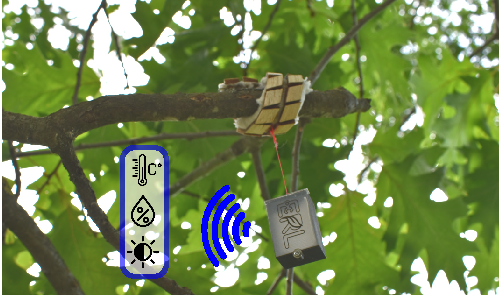
\includegraphics[width=1\columnwidth]{figures/figure1-overview/figure1-overview.pdf}
\caption{Biodegradable origami gripper attached to a tree branch. With rain, the gripper degrades and loses its grip, causing the sensor to fall to the ground.}
\label{fig1_overview_intro}
\end{figure}


The use of biodegradable sensors solves the problem of recovery, as the sensors simply decompose into harmless substances as they approach the end of their life cycle. Some promising work has been done towards fully biodegradable sensors and robots \cite{Sethi2022, Hartmann2021} with fully biodegradable components for batteries \cite{Yin2014, Wang2021, MicrobialCell}, actuators \cite{Baumgartner2020}, or structural components \cite{Wiesemuller2021Self-sensingStiffness, Hardman20213DStructures, Shintake2017}. Since the electronics needed for recording and transmitting data are most difficult to replicate with biodegradable materials, another approach is to develop sensors with active materials that react to changing environmental parameters with changes in shape or optical properties that can be sensed remotely \cite{Mazzolai2021} or remote reading of biodegradable sensors with passive RFID antennas \cite{Gopalakrishnan2022}. However, these approaches are still in the research and development stage, and not readily deployable in the field. A currently feasible approach are partially biodegradable hybrid systems, which contain biodegradable components, such as the attachment mechanisms, but conventional sensing, communication, and battery elements \cite{Sethi2022}. Biodegradable hybrid sensors can be deployed by aerial robots in the canopy and, once the strength of the biodegradable attachment weakens under the influence of environmental agents (e.g. humidity, light radiation, microbial activity, etc.), the sensors fall to the ground, facilitating the recovery of non-transitory components.

Therefore, in this work we investigate the development of a biodegradable gripper deployable by an aerial robot for sensor attachment to branches, see Fig. \ref{fig1_overview_intro}. The grasping principle is akin to that presented by the authors in \cite{Geckeler2022a}. The gripper consists of a bistable origami structure that transitions from an unfurled state, used for transport on a MAV, to the coiled state that wraps around the branch, see Fig. \ref{fig3_gripper_design}B. The transition is triggered when the MAV presses the gripper against the branch. In this work, all non-disposable materials used in the production of the original gripper \cite{Geckeler2022a} are replaced with biodegradable materials. In particular, the silicone elastomer required to produce the coiling force is replaced with a gelatin hydrogel, which, after sufficient exposure to moisture, degrades and releases the gripper from the branch. This drops the gripper and sensor to the ground, facilitating easier collection. This approach not only simplifies the recollection of the sensor, but also presents a more sustainable approach to robotics, both during manufacturing and after the robotic device has reached its end-of-life. Utilizing such biodegradable materials allows the mechanism to be disposed of without wasting precious resources or needing complicated recycling, and also induces less environmental strain during material generation and manufacturing.

The main contributions of this work are 1) analysis of materials for biodegradable origami, 2) development of a biodegradable origami gripper for sensor attachment, including outdoor deployment demonstration using a MAV, and 3) experimental characterization of the gripper as well as its actuating gelatin hydrogel, including the degradation behavior in the presence of moisture.

The rest of this paper is organized as follows, in Section II we detail our approach to biodegradable origami, including the biodegradable material selection, followed by the design of the gripper. Experimental characterization of the mechanical properties and degradation aspects of the gripper and the actuating gelatin hydrogel, and an outdoor aerial deployment follow in Section III. Section IV discusses the results and concludes the paper.


%%------------------------------------------------------------------------------------------------

\section{Biodegradable Origami}
% different from other approaches since not monolithic construction (which could be negative point)
Origami production lends itself well to the development of grippers for aerial use, as they are light, easy to produce and different gripping behaviours can be achieved by modifying the folding pattern \cite{Rus2018, Mintchev2018, Kim2018c}. Origami manufacturing utilizes a multi-layer composite of rigid and flexible layers, which when folded along the flexible joints can create complex 3D structures from planar sheets (Fig. \ref{fig2_biodegrad_layers}). The necessary components include a rigid layer, which provides structural integrity and determines the folding behavior, a flexible layer, which makes the joints, and an adhesive to bind the layers. In the origami gripper presented in \cite{Geckeler2022a}, the rigid layer is made with fiberglass, the flexible joints consist of a polyimide film and a heat- and pressure-activated adhesive (Pyralux® LF Bond Ply LF0111, DuPont) is used for bonding. A pre-stretched silicone elastomer is used as an actuating element for coiling the gripper around the branch. The conversion to a biodegradable origami gripper requires replacing all these materials. However, investigations into biodegradable origami is limited, \cite{Miyashita2015} showcases a controllable miniature origami robot, which is dissolvable in water, but not made from biodegradable components, and in \cite{Miyashita2016}, an ingestible origami robot for foreign body removal and stomach wound patching is presented. The materials utilized for the robot either lack the mechanical strength for outdoor deployment, or are biocompatible, but not biodegradable. Therefore, we first discuss potential biodegradable materials for origami fabrication, and then demonstrate their use in the coiling gripper.
\begin{figure}[!t]
\centering
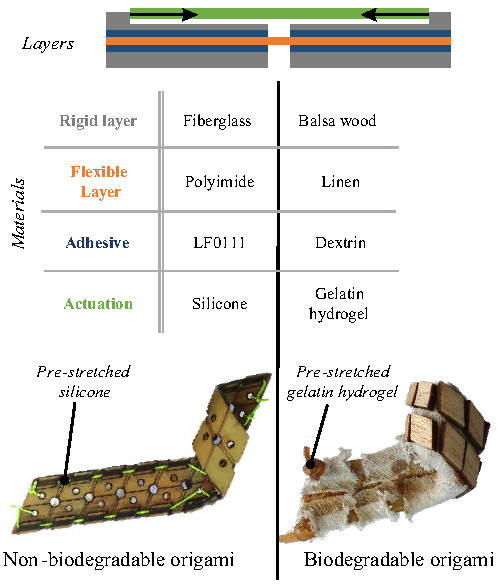
\includegraphics[width=1\columnwidth]{figures/figure2-biodegrad-layers/figure2-biodegrad-layers.pdf}
\caption{Biodegradable origami layers, with the gripper from \cite{Geckeler2022a} and its materials on the left, and the biodegradable gripper and materials on the right.}
\label{fig2_biodegrad_layers}
\end{figure}

\subsection{Material Selection}
A suitable biodegradable substitute must be found for each layer and component of the origami (Fig. \ref{fig2_biodegrad_layers}). For the selection, both the biodegradability of the material and its renewability were considered, with a preference for bio-derived, non fossil-based materials. The materials should be easily obtainable, affordable, lightweight, and easy to process to enable scalable aerially-deployed sensor systems.

Two possible options for the rigid layer are chitin- and cellulose-based materials. Chitin is a ubiquitous natural polymer found in the exoskeletons of crustaceans or insects. It is usable in a myriad of applications \cite{Elieh-Ali-Komi2016}, tough, and can also be used to cast complex 3D objects  \cite{Fernandez2014}.
Cellulose is an even more abundant biomaterial found primarily in the cells of plants, and is perhaps most familiar in the form of wood, paper, or cardboard, although it can also serve sensorized and structural purposes in robotics \cite{Wiesemuller2021Self-sensingStiffness, Mazzeo2021}. Due to its light weight, availability, ease of processing, and high strength-to-weight ratio, balsa wood was chosen as the rigid layer.

Similarly, the flexible layer also consists of cellulose fibers, in the form of linen cloth. Cloth was chosen since it has a high mechanical strength, suitability for repeated folding, and higher resistance to moisture than other cellulose-based sheet materials. Linen was chosen over other natural fibers such as cotton due to its reduced environmental footprint, requiring less water, energy, and pesticides to manufacture \cite{VanDerVelden2014LCAElastane, Shen2010EnvironmentalFibres}, as well as biodegrading faster \cite{Arshad2014}.

For adhesives there are several choices available, either starch or dextrin-based glues \cite{Radley1976}, animal glues such as gelatin, protein-based glues such as casein \cite{Bye1990} and soy protein-based glues \cite{Liu2002}, or bio-based epoxy resins \cite{Bassett2016}.
%glues:
% starch based glue
% dextrin (refined starch) based glue, maybe more viscose(?) (+ good for porous, slow curing, easy to manufacture
% animal-based glues (gelatin) (did not stick well to the linen?)
% Protein glues
% 	casein glue (milk-protein, water resistant (if add urea??)?, long setting time)
% 	soy-protein based glue (not easily available)
% bio-based epoxy resin (poor mechanical strength, not accessible, expensive)
Starch-based adhesives are completely biodegradable, provide a strong bond, and are well-studied for use in industrial packaging \cite{Maurer2009, Radley1976}. Therefore, a dextrin-based glue is chosen as an adhesive, since it is easy to source, very cheap, easy to manufacture from simple ingredients,  and easy to work with due to slow curing times.

The selection of a biodegradable elastomer with high elastic modulus as the actuating element is more challenging since even natural rubber degrades only slowly in nature \cite{Mahmoud2021ImprovementMonomers}. Gelatin-based hydrogels have shown promising results with high elasticity, fast biodegradation, and simple manufacturing \cite{Baumgartner2020, Hardman2022, Hardman20213DStructures, Shintake2017}.

% -	How to replace elements of origami gripper with biodegradable materials, need (also list avg. decomposition time for each): (also list alternatives for all)
%     - Flexible layer; linen (robust, stretchable, eco-friendly)
%     - Rigid layer; balsa wood (lightweight, robust)
%     - Adhesive; dextrin (simple to manufacture,)
%     - Elastic; gelatin (simple to manufacture, great elastic properties, high biodegradability)
    
\subsection{Biodegradable Origami Gripper}
\begin{figure}[!t]
\centering
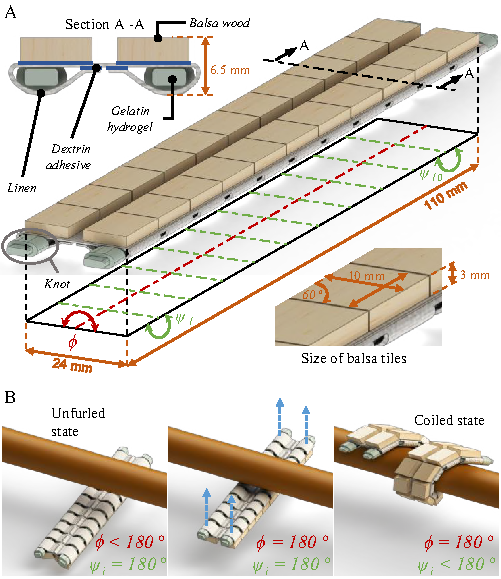
\includegraphics[width=1\columnwidth]{figures/figure3-gripper-design/figure3-gripper-design.pdf}%
\caption{Biodegradable origami gripper design. (A) Dimensions and materials for the origami gripper, the bottom side coils towards the branch. (B) Deployment process, left is the unfurled  transport state, folded along the red dashed line. Pressing against the branch (center) results in the coiled state (right), where the gripper is folded along the green dashed lines.}
\label{fig3_gripper_design}
\end{figure}

\subsubsection{Design and Working Principle}
The design and working principle of the gripper can be seen in Fig. \ref{fig3_gripper_design}A. The folding pattern consists of a single longitudinal fold (red dash-dot line) and ten transversal folds (green dash-dot lines). The folding pattern is obtained by attaching rhomboid balsa wood tiles to a layer of linen with a dextrin-based adhesive. The linen is then folded onto itself to create two channels through which the pre-stretched gelatin hydrogel is positioned. Knots on either end hold the gelatin in place and transmit contraction forces to the gripper, causing it to coil. The gripper has two stable states, the unfurled state (with $\phi < 180\degree$ and $\psi_i =180\degree$) which is the transport state used on the drone (Fig. \ref{fig3_gripper_design}B, left), and the coiled state for grasping (with $\phi = 180\degree$ and $\psi_i < 180\degree$, Fig. \ref{fig3_gripper_design}B, right). The state transition is initiated by pushing against a branch, which flattens the gripper until $\phi = 180\degree$ (Fig. \ref{fig3_gripper_design}B, center), at which point, the contraction forces applied by the pre-stretched gelatin hydrogel cause the gripper to coil around the branch. The biodegradable origami gripper is shorter but wider and thicker than the previous gripper, with a length of 110 mm, width of 24 mm, and 6.5 mm thickness. The reduced strength of balsa wood when compared to fiberglass requires a thicker rigid layer (3 mm vs. 0.3 mm). Additionally, since assembly, application of the adhesive, and bonding is done by hand, larger dimensions were chosen to facilitate manufacturing. 
For further details on the geometric characterization of the gripper the reader is referred to \cite{Geckeler2022a}. 

\subsubsection{Manufacturing}
Due to the selection of biodegradable materials, the biodegradable origami manufacturing process differs from conventional origami. In conventional origami the layers are usually laser-cut and bonded in a heat-press, whereas the biodegradable origami requires more manual intervention and a sequential approach since some materials are time-sensitive for curing. 

First, the balsa wood for the rigid layer is prepared. For a gripper with a length of 110 mm, twenty-two rhomboids with edge-lengths of 10 mm and an angle of 60\degree~ are cut out of 3 mm thick balsa wood. These are arranged in a plexiglass template, with two rows above each other and a 3 mm gap between the rows. This gap is the longitudinal joint, seen as the dash-dot red line in Fig. \ref{fig3_gripper_design}A. Next, the dextrin adhesive is prepared by mixing 21 g of de-ionized water, 1 g of glycerin, 0.5 g of glucose powder, and 13 g of dextrin in a hot water bath. This mixture is heated under constant mixing until it reaches 75 \degree C. The dextrin is produced by roasting commercial corn starch in the oven for 3 hours at 210 \degree C. The flexible layer can now be bonded to the rigid layer, for which an over-sized piece of linen is stretched taut and clamped, aligning the weave direction with the transversal cuts of the balsa wood. The dextrin adhesive is applied to the balsa wood pieces while still fluid, and clamped against the linen with even pressure, using the template. After curing, the channels for the gelatin hydrogel are prepared. In contrast with \cite{Geckeler2022a}, where the channels were also a multilayer composite of rigid and flexible layers, for the biodegradable gripper the channels are manufactured using solely the flexible layer. Excess strips of linen on both sides of the gripper are cut and looped back to create channels, with excess linen removed. These are then glued with another batch of prepared dextrin adhesive. The gripper is now prepared and ready for the gelatin hydrogel.

The composition of the gelatin hydrogel (G24) is similar to \cite{Baumgartner2020}, with 24 weight percent (wt\%) of gelatin (mesh 40 and bloom factor 260), 25.3 wt\% glucose, 32.5 wt\% glycerin (E422, 99.7\%), 14.5 wt\% de-ionized water, and 3.6 wt\% citric acid (E330). These materials are mixed under heat, then cast in a rectangular 2 mm thick plexiglass mold. This mold is first treated with a carnauba and soy wax releasing mixture \cite{Baumgartner2020} to prevent adhesion to the mold. The mold is oriented vertically such that most bubbles can rise, since a vacuum was not used. After cooling, the gelatin is laser-cut into the desired shapes, either dumbbell shapes for unixaxial tensile testing or the 150 mm long and 5 mm wide strips used for actuating the gripper.
To finish assembly of the gripper, the gelatin strips are lubricated with olive oil to ease their routing through the channels, fixed on one side with a knot, stretched to 1.4 - 1.9 strain, and fixed with another knot.

%%------------------------------------------------------------------------------------------------
\section{Experimental Characterization}
The two main parameters of interest for the gripper are the maximum holding force and its degradation with moisture. We first characterize the mechanical properties of the gelatin hydrogel, which provides the contractile force that drives the coiling of the gripper. We then measure the maximum weight the gripper can hold, which represents the maximum sensor payload and resistance to branch perturbations. We also characterize the amount of moisture required to release the gripper from the branch, indicating the amount of rain the gripper can endure before falling. % also water soluble, so also determines the degradation

\subsection{Gelatin Hydrogel Mechanical Characterization}

\begin{figure}[!t]
\centering
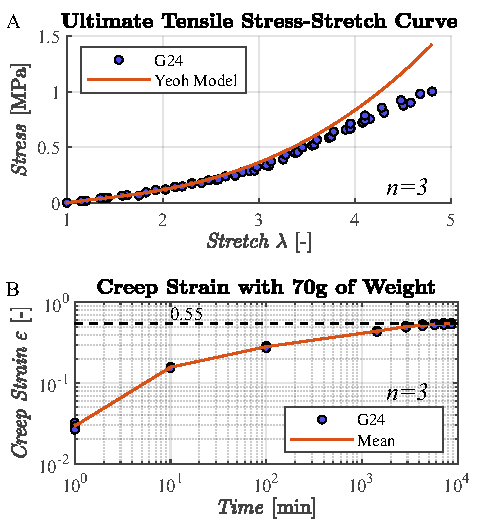
\includegraphics[width=1\columnwidth]{figures/figure4-gelatin_charac/figure4-gelatin-charac.pdf}%
\caption{Gelatin hydrogel material characterization. (A) Stress-stretch curve for the gelatin hydrogel, with the fitted Yeoh model. The gelatin dumbbell shapes were clamped into a similar setup to Fig. \ref{fig6_gripper_characterization} and stretched until break, logging the force. (B) Gelatin creep test, where 70 g were attached to one side of the gelatin and the elongation measured over six days.}
\label{fig4_gelatin_charac}
\end{figure}

Fig. \ref{fig4_gelatin_charac}A shows the stress-stretch curves for the material. For these tests a dumbbell shape according to the norm ISO: DIN 53504:2009-10 S2 was laser-cut from the G24 stock. One side of the sample was clamped to a load-cell, while the other was clamped to a linear rail. To reduce slippage, a clamping system for soft tissues \cite{Scholze2020} was used. Each sample was stretched uniaxially until break, with recording of the stress and visual post-processing of the video for strain. Fig.~\ref{fig4_gelatin_charac}A shows the data for three samples from one batch of gelatin, with the fitted Yeoh hyperelastic material model \cite{Shintake2017}. The Yeoh model stress is given by:
\begin{equation}
    S_{y} = 2(\lambda - \frac{1}{\lambda})\sum_{i=1}^3 iC_i(\lambda^2 + \frac{2}{\lambda} -3)^{i-1}
\label{yeoh_model}
\end{equation}
Where $\lambda$ is the uniaxial strain under assumption of incompressibility, and $C_i$ are material constants derived from fitting Equation~\ref{yeoh_model} to the measured data. The material constants are then used to estimate the Young's modulus. For derivations, see: \cite{Shintake2017, Yeoh1993SomeRubber}.
The ultimate tensile strength is 0.89 \textpm~0.13 N $(n=3)$, at a strain of 3.51 \textpm~0.33. The computed Young's modulus has a value of 0.12 \textpm~0.01 MPa, compared with 0.260 \textpm~0.060 from \cite{Baumgartner2020} (Table \ref{tab1_gelatin_charac}).


\begin{table}[!t]
% increase table row spacing, adjust to taste
\renewcommand{\arraystretch}{1.0}
% if using array.sty, it might be a good idea to tweak the value of
% \extrarowheight as needed to properly center the text within the cells
\caption{Ultimate Tensile Force, Strain, and Strength, Young's Modulus}
\label{tab1_gelatin_charac}
\centering
% Some packages, such as MDW tools, offer better commands for making tables
% than the plain LaTeX2e tabular which is used here.
\begin{tabular}{c|cccc}
& Force (N) & Strain (-) & Strength (MPa) & $E$ (MPa)\\
\hline
G24  & 7.27 \textpm~1.03 & 3.51 \textpm~0.33 & 0.89 \textpm~0.13 & 0.12 \textpm~0.01\\
\cite{Baumgartner2020} & - & 3.56 \textpm~0.11 & - & 0.260 \textpm~0.060\\
% \cite{Shintake2017} & - & - & 9.3 \textpm~1.2 & 2.7 \textpm~0.5\\ % different formula, so doesn't make sense to compare

\end{tabular}
\end{table}

% Yeoh model info/neo-hookian/ogden model

% To evaluate the elastic performance of the gelatin hydrogel over longer duration, creep tests were conducted.
Since the gripper will remain attached to the branch over longer periods of time, the elastic performance of the gelatin hydrogel over longer durations is of particular interest. If the gelatin displays large creep with a corresponding reduction in the contractile force, the gripping force of the gripper will also decrease, increasing the risk of the sensor falling. To quantify this behavior, creep tests were conducted by rigidly clamping one side of the samples and measuring the elongation of the material over a period of six days with a constant stress of 86.3 kPa applied to the sample (corresponding to a force of 0.69 N). The average creep over the 6 days for three samples can be seen in Fig. \ref{fig4_gelatin_charac}B. After a steep increase in elongation  within the first hour there is a plateau, with the maximum creep after the six days measuring 54.79 \textpm~1.31 \% $(n=3)$.


\subsection{Gripper Maximum Holding Force}
The test for the maximum holding force is illustrated in Fig. \ref{fig6_gripper_characterization}. The gripper is mounted on a test branch with a diameter of 18 mm, while a string attaches the gripper to a fixed load cell (Fig. \ref{fig6_gripper_characterization}A). The branch is moved upwards until the gripper disengages. The maximum holding force over five grippers was 1.03 \textpm~0.18 N. The maximum admissible payload of the gripper is therefore around 100 g for this branch diameter. This is well above the weight of the sensor and battery assembly from \cite{Geckeler2022a} of 8.55 g, providing a safety margin against creep, giving more robustness to external disturbances or allowing for larger and heavier sensors.

\begin{figure}[!t]
\centering
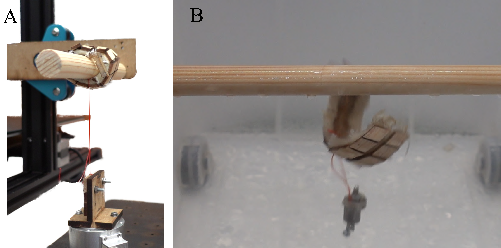
\includegraphics[width=1\columnwidth]{figures/figure6-gripper-charac/figure6-gripper-charac.pdf}
\caption{Gripper characterization. (A) Maximum holding force test, where the gripper can hold 1.08 \textpm~0.18 N $(n=5)$. (B) Gripper falling after being sprayed with 10.48 \textpm~2.92 ml $(n=3)$ of water.}
\label{fig6_gripper_characterization}
\end{figure}

\subsection{Degradation}

\begin{figure}[!t]
\centering
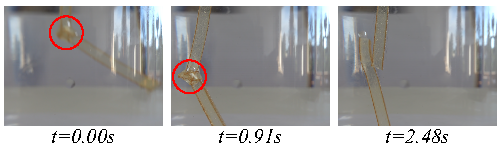
\includegraphics[width=1\columnwidth]{figures/figure5-gelatin-degrade/figure5-gelatin-degrade.pdf}
\caption{A submerged gelatin knot dissolving within seconds, average time to dissolve is 3.6 \textpm~2.88 seconds $(n=3)$.}
\label{fig5_gelatin_degrade}
\end{figure}
To facilitate the dropping of the sensor, a suitable degradation method must be chosen. Degradation could be enzymatic \cite{Arshad2014}, induced by exposure to ultraviolet (UV) radiation, or moisture. Since microbes are less present on tree branches than in soil and the attachment location could be sheltered from UV exposure, moisture was chosen as a fast-acting and ubiquitous degradation solution.
Both the dextrin adhesive and the gelatin hydrogel are water-soluble and present potential vectors for degradation in the presence of moisture. To determine which dissolves faster and will be the limiting factor, solid pieces of both were immersed in de-ionized water. While only the surface of the dextrin dissolved faster, the gelatin absorbed the water, remaining structurally intact, but lacking mechanical strength and falling apart with a slight disturbance. 

Since the materials will be under tension in the gripper, loaded dissolution tests were performed next. The adhesion of linen to linen with dextrin was tested by adhering two strips of linen, fixing one end and weighing down the other before immersion in water. Linen to balsa wood with dextrin was tested by weighing down the linen and letting the balsa wood float. The dextrin samples for linen to linen held four minutes and 18 minutes for linen to balsa wood. To simulate tension in the gelatin, strips of gelatin with a knot were submerged in water. Within seconds (3.6 \textpm~2.88 seconds, Fig. \ref{fig5_gelatin_degrade}) the gelatin in the knot had dissolved and the strip had been split. Therefore the gelatin loses mechanical integrity much faster than the dextrin adhesive when under tension. When compared with unloaded strips of gelatin, the knot dissolved magnitudes faster, indicating that higher and more localized mechanical stress leads to faster degradation.
Since the gelatin must be under tension for the gripper to remain attached, degradation of the gelatin hydrogel under sufficient exposure to moisture will cause the gripper to fall.
% The mechanical characteristics of the gelatin hydrogel also  directly determine gripper holding strength. Since both gripper strength and duration until degradation are directly influenced by the gelatin hydrogel, its properties are analyzed in further detail here.
% local stresses dissolve first (knot), can either be bad, so that next time fasten gelatin differently, of positive, since it can be precise point of failure.

Next, the quantity of water needed for the fully assembled gripper to  fall was measured, see Fig. \ref{fig6_gripper_characterization}B. In these experiments the gripper was weighed down with 20 g, then 0.17 ml of water were sprayed on the gripper at 30 second time intervals, simulating a precipitation of 490 ml/day. The three sample grippers were able to withstand on average 10.48 \textpm~2.92 ml of water before falling, measured as the quantity of water impacting the area of the gripper. The time before failure was 31 \textpm~8 minutes. For every sample the point of failure was the knot of gelatin keeping the gelatin at the desired strain, which is also the area experiencing the most localized tension. When the knot gives way, the gelatin no longer provides the contractile force required for coiling, causing the gripper to fall.

Finally, we exposed a gripper to a considerably lower precipitation rate of 0.68 ml/day (we sprayed 0.68 ml of water every day). In this test the 
gripper was able to withstand 3.4 ml of water, but remained attached to the branch for five days before falling. This shows that the gripper is capable of sustaining a reduced volume of water exposure over an extended time before failure, such as a longer drizzle rain, or a high humidity environment. This makes the gripper particularly suitable for use cases such as studying the effects of droughts in forests. The gripper would remain attached and monitor during the dry weeks, and once it rains it would fall and be ready for collection.
%
%The grippers sustained 10.48 \textpm~2.92 ml of water before falling, which is equivalent to 3.36 \textpm~0.85 mm of precipitation, normalized to the amount of water only hitting the gripper area. This makes the gripper particularly suitable for use cases such as studying the effects of droughts in forests. The gripper would remain attached and monitor during the dry weeks, and once it rains it would fall and be ready for collection. To increase the gripper's versatility, it could be beneficial to control its resistance to degradation until failure. Therefore, future work will investigate tuning of the gelatin hydrogel to adjust its hydrophilicity and thereby the degradation rate. Water resistance can be increased through the addition of different cross-linking agents to the gelatin \cite{Biscarat2015, Gomez-Estaca2011, Ahammed2020, Chaochai2016, Wang2020}, adding a coating to the gelatin hydrogel after manufacture \cite{Chen2018}, or both \cite{Stoessel2015}.
%
%This volume of water will cause the gripper to fall in a short time period, 31 \textpm~8 minutes. However, to show that the gripper will remain attached for longer periods of time when exposed to smaller quantities of water, a gripper is sprayed with 0.68 ml per day and lasts for five days before it falls. This shows that the gripper is capable of sustaining a reduced volume of water exposure over an extended time before failure, such as a longer drizzle rain, or a high humidity environment. 
% This volume of water will cause the gripper to fail immediately, however, it is assumed that with lower quantities of water dispersal the gripper will remain attached longer. To demonstrate that the gripper will not fail prematurely, a gripper is sprayed with 0.68 ml per day for five days before it falls, compared with 31 minutes to failure for the previous test. This shows that the gripper is capable of sustaining a reduced volume of water exposure, but for an extended time before failure, such as a longer drizzle rain, or a high humidity environment. 
% % Not really, there is no "recovery" once the gelatin gets wet it starts to fail, regardless of how much water is sprayed
%
\subsection{Sensor Delivery}
The same drone platform based on a DJI Mavic Mini with an added collision protection net as in \cite{Geckeler2022a} was used to deploy the gripper (Fig. \ref{fig7_outdoor}A). Previously, magnets held the gripper in place on the drone and released once the gripper began to coil. To avoid the non-biodegradable magnets, a simple clamping mechanism was developed (Fig. \ref{fig7_outdoor}B), which holds the gripper in the unfurled state and releases it after contact with the branch. Two flexible 3D-printed U-shaped holders are tightened with an elastic, allowing the gripper to be clamped. Contact with the branch in the center of the gripper causes it to coil, releasing the ends from the clamps. The deployment process of the biodegradable gripper remains the same, a rapid upwards motion clasps the gripper around the branch and attaches it, as can be seen in Fig. \ref{fig7_outdoor}. Once the gripper is attached the sensors can begin measuring data, contained within the sensor box (Fig. \ref{fig1_overview_intro}) is a TinyDunio with Combo Sensor Tinyshield and a 150mAh battery, measuring temperature, humidity, barometric pressure, ambient light, and sensor attitude with an IMU.
\begin{figure}[!t]
\centering
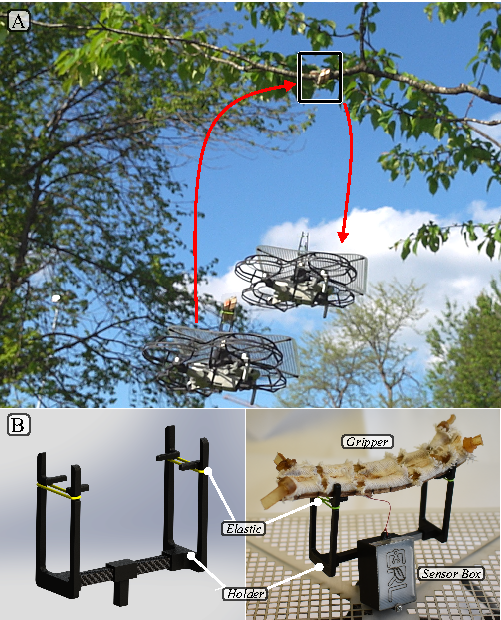
\includegraphics[width=1\columnwidth]{figures/figure7-outdoor/figure7-outdoor.pdf}
\caption{(A) Outdoor deployment of the biodegradable gripper with a MAV. (B) Left - CAD render of the new gripper holder. Right - Biodegradable gripper with sensor box attached to the drone.}
\label{fig7_outdoor}
\end{figure}

%\section{Discussion}
%The gelatin hydrogel defines the two most important properties of the gripper, the holding force and its degradation behaviour. Since the gelatin provides the contractile force required for coiling, it directly determines the holding force of the gripper. Similarly, after exposure to moisture, gelatin was shown to lose mechanical functioning the quickest, and therefore also determines the degradation behaviour of the gripper.
%In order to reduce the loss of force due to creep (Fig. \ref{fig4_gelatin_charac}B) or increase the contractile force, the mechanical properties of the hydorgel could be improved. To do so, 
%utilizing a vacuum pump during manufacturing would greatly reduce the amount of bubbles and increase material homogeneity and strength. In \cite{Heiden2022} it is shown that 3D printing gelatin hydrogels results in higher elastic moduli when compared to casting, which could also improve performance. 
%The grippers sustained 10.48 \textpm~2.92 ml of water before falling, which is equivalent to 3.36 \textpm~0.85 mm of precipitation, normalized to the amount of water only hitting the gripper area. This makes the gripper particularly suitable for use cases such as studying the effects of droughts in forests. The gripper would remain attached and monitor during the dry weeks, and once it rains it would fall and be ready for collection. To increase the gripper's versatility, it could be beneficial to control this duration until failure. Therefore, future work will investigate tuning of the gelatin hydrogel to adjust its hydrophilicity and thereby the degradation time. Water resistance can be increased through the addition of different cross-linking agents to the gelatin \cite{Biscarat2015, Gomez-Estaca2011, Ahammed2020, Chaochai2016, Wang2020}, adding a coating to the gelatin hydrogel after manufacture \cite{Chen2018}, or both \cite{Stoessel2015}.

%%------------------------------------------------------------------------------------------------
\section{Conclusion}
In this work we developed a MAV-deployable biodegradable origami gripper for sensor attachment to tree branches. A suitable biodegradable replacement was selected for each of the origami components; with balsa wood as the rigid layer, linen for the flexible layer, a dextrin-based glue as the adhesive, and a gelatin-based hydrogel as the elastic actuator. The pre-stretched gelatin hydrogel allows the gripper to hold up to 1 N, which is sufficient to fix a sensor payload of 10 g, even though the gelatin creep decreases the holding force over time. It was also determined that the gelatin would serve as the degradation point, with the knots being the failure point. It is shown that the knots of the gelatin hydrogel will degrade and drop the gripper after water is dispersed on the gripper. Depending on the precipitation rate, the gripper can absorb up to 10 ml of water and resist for five days before falling off a branch. Deployment of the gripper with a MAV is also demonstrated.

To increase the gripper's versatility, it could be beneficial to control its resistance to degradation until failure. Therefore, future work will investigate tuning of the gelatin hydrogel to adjust its hydrophilicity and thereby the degradation rate. Water resistance can be increased through the addition of different cross-linking agents to the gelatin \cite{Biscarat2015, Gomez-Estaca2011, Ahammed2020, Chaochai2016, Wang2020}, adding a coating to the gelatin hydrogel after manufacture \cite{Chen2018}, or both \cite{Stoessel2015}. Investigating outdoor environmental variables, such as temperature or presence of microbes, on the degradation process would also be of interest. Once the gelatin degrades, the gripper releases and should fall to the ground with the sensor. Entanglement with lower branches is not considered, since it is assumed that with enough perturbations from wind eventually the gripper will reach the ground, although this needs to be empirically verified. While collecting sensors from the ground is easier than from tree canopies, it is still not a trivial task. Utilizing large electromagnets to recollect the sensors \cite{Iyer2022} still requires proximity with the sensor, which could be achieved by locating sensors with the help of radio, WiFi, Bluetooth or other broadcasting capabilities emanating from the sensor. Finally, through the simple addition of NaCl, the gelatin hydrogel could also function as a strain sensor \cite{Hardman2022}, which could then be used to infer information about the status of coiling or the diameter of branch the gripper is placed on.

Overall, the biodegradable origami gripper represents a more scalable and environmentally sustainable approach towards ecosystem monitoring, a first step towards the long-term goal of fully biodegradable sensors. Further in the future, we envision fully biodegradable sensors which allow for remote determination of environmental parameters without re-collection of the sensor.
%%------------------------------------------------------------------------------------------------

% \addtolength{\textheight}{-12cm}   % This command serves to balance the column lengths
%                                   % on the last page of the document manually. It shortens
%                                   % the textheight of the last page by a suitable amount.
%                                   % This command does not take effect until the next page
%                                   % so it should come on the page before the last. Make
%                                   % sure that you do not shorten the textheight too much.

%%%%%%%%%%%%%%%%%%%%%%%%%%%%%%%%%%%%%%%%%%%%%%%%%%%%%%%%%%%%%%%%%%%%%%%%%%%%%%%%



%%%%%%%%%%%%%%%%%%%%%%%%%%%%%%%%%%%%%%%%%%%%%%%%%%%%%%%%%%%%%%%%%%%%%%%%%%%%%%%%



% %%%%%%%%%%%%%%%%%%%%%%%%%%%%%%%%%%%%%%%%%%%%%%%%%%%%%%%%%%%%%%%%%%%%%%%%%%%%%%%%
% \section*{APPENDIX}

% Appendixes should appear before the acknowledgment.

\section*{Acknowledgments}
The authors would like to thank Biogel AG for graciously providing the gelatin.



%%%%%%%%%%%%%%%%%%%%%%%%%%%%%%%%%%%%%%%%%%%%%%%%%%%%%%%%%%%%%%%%%%%%%%%%%%%%%%%%
